\documentclass[10pt,usepdftitle=false,aspectratio=169]{beamer}



% Preamble
%!TEX root = talk.tex


% Fonts and encoding
\usepackage[utf8]{inputenc} % allow utf-8 input
\usepackage[T1]{fontenc}    % use 8-bit T1 fonts
\usepackage{microtype}      % microtypography
\usepackage{inconsolata}
\usepackage[sfdefault,light,condensed]{roboto}
\usefonttheme[onlymath]{serif} % serif fonts for mathematics

% Enumerations and Items
\usepackage{fourier-orns} % starred bullets
% \usepackage{enumitem}


% Mathematics and Notation
\usepackage{amsmath}
\usepackage{amssymb}
\usepackage{amsfonts}       % blackboard math symbols
\usepackage{nicefrac}       % compact symbols for 1/2, etc.
\usepackage{mathtools}
\usepackage{bm}
\usepackage{physics}
% (Adjusted) mathematics commands from https://github.com/goodfeli/dlbook_notation.
%%%%% NEW MATH DEFINITIONS %%%%%

\usepackage{amsmath,amsfonts,bm}

% Mark sections of captions for referring to divisions of figures
\newcommand{\figleft}{{\em (Left)}}
\newcommand{\figcenter}{{\em (Center)}}
\newcommand{\figright}{{\em (Right)}}
\newcommand{\figtop}{{\em (Top)}}
\newcommand{\figbottom}{{\em (Bottom)}}
\newcommand{\captiona}{{\em (a)}}
\newcommand{\captionb}{{\em (b)}}
\newcommand{\captionc}{{\em (c)}}
\newcommand{\captiond}{{\em (d)}}

% Highlight a newly defined term
\newcommand{\newterm}[1]{{\bf #1}}


% Figure reference, lower-case.
\def\figref#1{figure~\ref{#1}}
% Figure reference, capital. For start of sentence
\def\Figref#1{Figure~\ref{#1}}
\def\twofigref#1#2{figures \ref{#1} and \ref{#2}}
\def\quadfigref#1#2#3#4{figures \ref{#1}, \ref{#2}, \ref{#3} and \ref{#4}}
% Section reference, lower-case.
\def\secref#1{section~\ref{#1}}
% Section reference, capital.
\def\Secref#1{Section~\ref{#1}}
% Reference to two sections.
\def\twosecrefs#1#2{sections \ref{#1} and \ref{#2}}
% Reference to three sections.
\def\secrefs#1#2#3{sections \ref{#1}, \ref{#2} and \ref{#3}}
% Reference to an equation, lower-case.
%\def\eqref#1{equation~\ref{#1}}
% Reference to an equation, upper case
%\def\Eqref#1{Equation~\ref{#1}}
% A raw reference to an equation---avoid using if possible
\def\plaineqref#1{\ref{#1}}
% Reference to a chapter, lower-case.
\def\chapref#1{chapter~\ref{#1}}
% Reference to an equation, upper case.
\def\Chapref#1{Chapter~\ref{#1}}
% Reference to a range of chapters
\def\rangechapref#1#2{chapters\ref{#1}--\ref{#2}}
% Reference to an algorithm, lower-case.
\def\algref#1{algorithm~\ref{#1}}
% Reference to an algorithm, upper case.
\def\Algref#1{Algorithm~\ref{#1}}
\def\twoalgref#1#2{algorithms \ref{#1} and \ref{#2}}
\def\Twoalgref#1#2{Algorithms \ref{#1} and \ref{#2}}
% Reference to a part, lower case
\def\partref#1{part~\ref{#1}}
% Reference to a part, upper case
\def\Partref#1{Part~\ref{#1}}
\def\twopartref#1#2{parts \ref{#1} and \ref{#2}}

\def\ceil#1{\lceil #1 \rceil}
\def\floor#1{\lfloor #1 \rfloor}
\def\1{\bm{1}}
\newcommand{\train}{\mathcal{D}}
\newcommand{\valid}{\mathcal{D_{\mathrm{valid}}}}
\newcommand{\test}{\mathcal{D_{\mathrm{test}}}}

\def\eps{{\epsilon}}


% Random variables
\def\reta{{\mathsf{$\eta$}}}
\def\ra{{\mathsf{a}}}
\def\rb{{\mathsf{b}}}
\def\rc{{\mathsf{c}}}
\def\rd{{\mathsf{d}}}
\def\re{{\mathsf{e}}}
\def\rf{{\mathsf{f}}}
\def\rg{{\mathsf{g}}}
\def\rh{{\mathsf{h}}}
\def\ri{{\mathsf{i}}}
\def\rj{{\mathsf{j}}}
\def\rk{{\mathsf{k}}}
\def\rl{{\mathsf{l}}}
% rm is already a command, just don't name any random variables m
\def\rn{{\mathsf{n}}}
\def\ro{{\mathsf{o}}}
\def\rp{{\mathsf{p}}}
\def\rq{{\mathsf{q}}}
\def\rr{{\mathsf{r}}}
\def\rs{{\mathsf{s}}}
\def\rt{{\mathsf{t}}}
\def\ru{{\mathsf{u}}}
\def\rv{{\mathsf{v}}}
\def\rw{{\mathsf{w}}}
\def\rx{{\mathsf{x}}}
\def\ry{{\mathsf{y}}}
\def\rz{{\mathsf{z}}}

% Random vectors
\def\rvepsilon{{\bm{\mathsf{\epsilon}}}}
\def\rvtheta{{\bm{\mathsf{\theta}}}}
\def\rva{{\bm{\mathsf{a}}}}
\def\rvb{{\bm{\mathsf{b}}}}
\def\rvc{{\bm{\mathsf{c}}}}
\def\rvd{{\bm{\mathsf{d}}}}
\def\rve{{\bm{\mathsf{e}}}}
\def\rvf{{\bm{\mathsf{f}}}}
\def\rvg{{\bm{\mathsf{g}}}}
\def\rvh{{\bm{\mathsf{h}}}}
\def\rvu{{\bm{\mathsf{i}}}}
\def\rvj{{\bm{\mathsf{j}}}}
\def\rvk{{\bm{\mathsf{k}}}}
\def\rvl{{\bm{\mathsf{l}}}}
\def\rvm{{\bm{\mathsf{m}}}}
\def\rvn{{\bm{\mathsf{n}}}}
\def\rvo{{\bm{\mathsf{o}}}}
\def\rvp{{\bm{\mathsf{p}}}}
\def\rvq{{\bm{\mathsf{q}}}}
\def\rvr{{\bm{\mathsf{r}}}}
\def\rvs{{\bm{\mathsf{s}}}}
\def\rvt{{\bm{\mathsf{t}}}}
\def\rvu{{\bm{\mathsf{u}}}}
\def\rvv{{\bm{\mathsf{v}}}}
\def\rvw{{\bm{\mathsf{w}}}}
\def\rvx{{\bm{\mathsf{x}}}}
\def\rvy{{\bm{\mathsf{y}}}}
\def\rvz{{\bm{\mathsf{z}}}}

% Elements of random vectors
\def\erva{\bm{\mathsf{a}}}
\def\ervb{\bm{\mathsf{b}}}
\def\ervc{\bm{\mathsf{c}}}
\def\ervd{{\mathsf{d}}}
\def\erve{{\mathsf{e}}}
\def\ervf{{\mathsf{f}}}
\def\ervg{{\mathsf{g}}}
\def\ervh{{\mathsf{h}}}
\def\ervi{{\mathsf{i}}}
\def\ervj{{\mathsf{j}}}
\def\ervk{{\mathsf{k}}}
\def\ervl{{\mathsf{l}}}
\def\ervm{{\mathsf{m}}}
\def\ervn{{\mathsf{n}}}
\def\ervo{{\mathsf{o}}}
\def\ervp{{\mathsf{p}}}
\def\ervq{{\mathsf{q}}}
\def\ervr{{\mathsf{r}}}
\def\ervs{{\mathsf{s}}}
\def\ervt{{\mathsf{t}}}
\def\ervu{{\mathsf{u}}}
\def\ervv{{\mathsf{v}}}
\def\ervw{{\mathsf{w}}}
\def\ervx{{\mathsf{x}}}
\def\ervy{{\mathsf{y}}}
\def\ervz{{\mathsf{z}}}

% Random matrices
\def\rmA{{\bm{\mathsf{A}}}}
\def\rmB{{\bm{\mathsf{B}}}}
\def\rmC{{\bm{\mathsf{C}}}}
\def\rmD{{\bm{\mathsf{D}}}}
\def\rmE{{\bm{\mathsf{E}}}}
\def\rmF{{\bm{\mathsf{F}}}}
\def\rmG{{\bm{\mathsf{G}}}}
\def\rmH{{\bm{\mathsf{H}}}}
\def\rmI{{\bm{\mathsf{I}}}}
\def\rmJ{{\bm{\mathsf{J}}}}
\def\rmK{{\bm{\mathsf{K}}}}
\def\rmL{{\bm{\mathsf{L}}}}
\def\rmM{{\bm{\mathsf{M}}}}
\def\rmN{{\bm{\mathsf{N}}}}
\def\rmO{{\bm{\mathsf{O}}}}
\def\rmP{{\bm{\mathsf{P}}}}
\def\rmQ{{\bm{\mathsf{Q}}}}
\def\rmR{{\bm{\mathsf{R}}}}
\def\rmS{{\bm{\mathsf{S}}}}
\def\rmT{{\bm{\mathsf{T}}}}
\def\rmU{{\bm{\mathsf{U}}}}
\def\rmV{{\bm{\mathsf{V}}}}
\def\rmW{{\bm{\mathsf{W}}}}
\def\rmX{{\bm{\mathsf{X}}}}
\def\rmY{{\bm{\mathsf{Y}}}}
\def\rmZ{{\bm{\mathsf{Z}}}}
\def\rmBeta{{\bm{\mathsf{\beta}}}}
\def\rmPi{{\bm{\mathsf{\Pi}}}}
\def\rmPhi{{\bm{\mathsf{\Phi}}}}
\def\rmPsi{{\bm{\mathsf{\Psi}}}}
\def\rmLambda{{\bm{\mathsf{\Lambda}}}}
\def\rmSigma{{\bm{\mathsf{\Sigma}}}}
\def\rmDelta{{\bm{\mathsf{\Delta}}}}

% Elements of random matrices
\def\ermA{{\mathsf{A}}}
\def\ermB{{\mathsf{B}}}
\def\ermC{{\mathsf{C}}}
\def\ermD{{\mathsf{D}}}
\def\ermE{{\mathsf{E}}}
\def\ermF{{\mathsf{F}}}
\def\ermG{{\mathsf{G}}}
\def\ermH{{\mathsf{H}}}
\def\ermI{{\mathsf{I}}}
\def\ermJ{{\mathsf{J}}}
\def\ermK{{\mathsf{K}}}
\def\ermL{{\mathsf{L}}}
\def\ermM{{\mathsf{M}}}
\def\ermN{{\mathsf{N}}}
\def\ermO{{\mathsf{O}}}
\def\ermP{{\mathsf{P}}}
\def\ermQ{{\mathsf{Q}}}
\def\ermR{{\mathsf{R}}}
\def\ermS{{\mathsf{S}}}
\def\ermT{{\mathsf{T}}}
\def\ermU{{\mathsf{U}}}
\def\ermV{{\mathsf{V}}}
\def\ermW{{\mathsf{W}}}
\def\ermX{{\mathsf{X}}}
\def\ermY{{\mathsf{Y}}}
\def\ermZ{{\mathsf{Z}}}

% Vectors
\def\vzero{{\bm{0}}}
\def\vone{{\bm{1}}}
\def\vmu{{\bm{\mu}}}
\def\vtheta{{\bm{\theta}}}
\def\valpha{{\bm{\alpha}}}
\def\vbeta{{\bm{\beta}}}
\def\vgamma{{\bm{\gamma}}}
\def\vlambda{{\bm{\lambda}}}
\def\vphi{{\bm{\phi}}}
\def\vpsi{{\bm{\psi}}}
\def\vxi{{\bm{\xi}}}
\def\va{{\bm{a}}}
\def\vb{{\bm{b}}}
\def\vc{{\bm{c}}}
\def\vd{{\bm{d}}}
\def\ve{{\bm{e}}}
\def\vf{{\bm{f}}}
\def\vg{{\bm{g}}}
\def\vh{{\bm{h}}}
\def\vi{{\bm{i}}}
\def\vj{{\bm{j}}}
\def\vk{{\bm{k}}}
\def\vl{{\bm{l}}}
\def\vm{{\bm{m}}}
\def\vn{{\bm{n}}}
\def\vo{{\bm{o}}}
\def\vp{{\bm{p}}}
\def\vq{{\bm{q}}}
\def\vr{{\bm{r}}}
\def\vs{{\bm{s}}}
\def\vt{{\bm{t}}}
\def\vu{{\bm{u}}}
\def\vv{{\bm{v}}}
\def\vw{{\bm{w}}}
\def\vx{{\bm{x}}}
\def\vy{{\bm{y}}}
\def\vz{{\bm{z}}}

% Elements of vectors
\def\evalpha{{\alpha}}
\def\evbeta{{\beta}}
\def\evepsilon{{\epsilon}}
\def\evlambda{{\lambda}}
\def\evomega{{\omega}}
\def\evmu{{\mu}}
\def\evpsi{{\psi}}
\def\evsigma{{\sigma}}
\def\evtheta{{\theta}}
\def\evphi{{\phi}}
\def\evxi{{\xi}}
\def\eva{{a}}
\def\evb{{b}}
\def\evc{{c}}
\def\evd{{d}}
\def\eve{{e}}
\def\evf{{f}}
\def\evg{{g}}
\def\evh{{h}}
\def\evi{{i}}
\def\evj{{j}}
\def\evk{{k}}
\def\evl{{l}}
\def\evm{{m}}
\def\evn{{n}}
\def\evo{{o}}
\def\evp{{p}}
\def\evq{{q}}
\def\evr{{r}}
\def\evs{{s}}
\def\evt{{t}}
\def\evu{{u}}
\def\evv{{v}}
\def\evw{{w}}
\def\evx{{x}}
\def\evy{{y}}
\def\evz{{z}}

% Matrix
\def\mA{{\bm{A}}}
\def\mB{{\bm{B}}}
\def\mC{{\bm{C}}}
\def\mD{{\bm{D}}}
\def\mE{{\bm{E}}}
\def\mF{{\bm{F}}}
\def\mG{{\bm{G}}}
\def\mH{{\bm{H}}}
\def\mI{{\bm{I}}}
\def\mJ{{\bm{J}}}
\def\mK{{\bm{K}}}
\def\mL{{\bm{L}}}
\def\mM{{\bm{M}}}
\def\mN{{\bm{N}}}
\def\mO{{\bm{O}}}
\def\mP{{\bm{P}}}
\def\mQ{{\bm{Q}}}
\def\mR{{\bm{R}}}
\def\mS{{\bm{S}}}
\def\mT{{\bm{T}}}
\def\mU{{\bm{U}}}
\def\mV{{\bm{V}}}
\def\mW{{\bm{W}}}
\def\mX{{\bm{X}}}
\def\mY{{\bm{Y}}}
\def\mZ{{\bm{Z}}}
\def\mBeta{{\bm{\beta}}}
\def\mPi{{\bm{\Pi}}}
\def\mPhi{{\bm{\Phi}}}
\def\mPsi{{\bm{\Psi}}}
\def\mLambda{{\bm{\Lambda}}}
\def\mSigma{{\bm{\Sigma}}}
\def\mDelta{{\bm{\Delta}}}

% Tensor
\DeclareMathAlphabet{\mathsfit}{\encodingdefault}{\sfdefault}{m}{sl}
\SetMathAlphabet{\mathsfit}{bold}{\encodingdefault}{\sfdefault}{bx}{n}
\newcommand{\tens}[1]{\bm{\mathsfit{#1}}}
\def\tA{{\tens{A}}}
\def\tB{{\tens{B}}}
\def\tC{{\tens{C}}}
\def\tD{{\tens{D}}}
\def\tE{{\tens{E}}}
\def\tF{{\tens{F}}}
\def\tG{{\tens{G}}}
\def\tH{{\tens{H}}}
\def\tI{{\tens{I}}}
\def\tJ{{\tens{J}}}
\def\tK{{\tens{K}}}
\def\tL{{\tens{L}}}
\def\tM{{\tens{M}}}
\def\tN{{\tens{N}}}
\def\tO{{\tens{O}}}
\def\tP{{\tens{P}}}
\def\tQ{{\tens{Q}}}
\def\tR{{\tens{R}}}
\def\tS{{\tens{S}}}
\def\tT{{\tens{T}}}
\def\tU{{\tens{U}}}
\def\tV{{\tens{V}}}
\def\tW{{\tens{W}}}
\def\tX{{\tens{X}}}
\def\tY{{\tens{Y}}}
\def\tZ{{\tens{Z}}}


% Graph
\def\gA{{\mathcal{A}}}
\def\gB{{\mathcal{B}}}
\def\gC{{\mathcal{C}}}
\def\gD{{\mathcal{D}}}
\def\gE{{\mathcal{E}}}
\def\gF{{\mathcal{F}}}
\def\gG{{\mathcal{G}}}
\def\gH{{\mathcal{H}}}
\def\gI{{\mathcal{I}}}
\def\gJ{{\mathcal{J}}}
\def\gK{{\mathcal{K}}}
\def\gL{{\mathcal{L}}}
\def\gM{{\mathcal{M}}}
\def\gN{{\mathcal{N}}}
\def\gO{{\mathcal{O}}}
\def\gP{{\mathcal{P}}}
\def\gQ{{\mathcal{Q}}}
\def\gR{{\mathcal{R}}}
\def\gS{{\mathcal{S}}}
\def\gT{{\mathcal{T}}}
\def\gU{{\mathcal{U}}}
\def\gV{{\mathcal{V}}}
\def\gW{{\mathcal{W}}}
\def\gX{{\mathcal{X}}}
\def\gY{{\mathcal{Y}}}
\def\gZ{{\mathcal{Z}}}

% Sets
\def\sA{{\mathbb{A}}}
\def\sB{{\mathbb{B}}}
\def\sC{{\mathbb{C}}}
\def\sD{{\mathbb{D}}}
% Don't use a set called E, because this would be the same as our symbol
% for expectation.
\def\sF{{\mathbb{F}}}
\def\sG{{\mathbb{G}}}
\def\sH{{\mathbb{H}}}
\def\sI{{\mathbb{I}}}
\def\sJ{{\mathbb{J}}}
\def\sK{{\mathbb{K}}}
\def\sL{{\mathbb{L}}}
\def\sM{{\mathbb{M}}}
\def\sN{{\mathbb{N}}}
\def\sO{{\mathbb{O}}}
\def\sP{{\mathbb{P}}}
\def\sQ{{\mathbb{Q}}}
\def\sR{{\mathbb{R}}}
\def\sS{{\mathbb{S}}}
\def\sT{{\mathbb{T}}}
\def\sU{{\mathbb{U}}}
\def\sV{{\mathbb{V}}}
\def\sW{{\mathbb{W}}}
\def\sX{{\mathbb{X}}}
\def\sY{{\mathbb{Y}}}
\def\sZ{{\mathbb{Z}}}

% Entries of a matrix
\def\emLambda{{\Lambda}}
\def\emA{{A}}
\def\emB{{B}}
\def\emC{{C}}
\def\emD{{D}}
\def\emE{{E}}
\def\emF{{F}}
\def\emG{{G}}
\def\emH{{H}}
\def\emI{{I}}
\def\emJ{{J}}
\def\emK{{K}}
\def\emL{{L}}
\def\emM{{M}}
\def\emN{{N}}
\def\emO{{O}}
\def\emP{{P}}
\def\emQ{{Q}}
\def\emR{{R}}
\def\emS{{S}}
\def\emT{{T}}
\def\emU{{U}}
\def\emV{{V}}
\def\emW{{W}}
\def\emX{{X}}
\def\emY{{Y}}
\def\emZ{{Z}}
\def\emSigma{{\Sigma}}

% entries of a tensor
% Same font as tensor, without \bm wrapper
\newcommand{\etens}[1]{\mathsfit{#1}}
\def\etLambda{{\etens{\Lambda}}}
\def\etA{{\etens{A}}}
\def\etB{{\etens{B}}}
\def\etC{{\etens{C}}}
\def\etD{{\etens{D}}}
\def\etE{{\etens{E}}}
\def\etF{{\etens{F}}}
\def\etG{{\etens{G}}}
\def\etH{{\etens{H}}}
\def\etI{{\etens{I}}}
\def\etJ{{\etens{J}}}
\def\etK{{\etens{K}}}
\def\etL{{\etens{L}}}
\def\etM{{\etens{M}}}
\def\etN{{\etens{N}}}
\def\etO{{\etens{O}}}
\def\etP{{\etens{P}}}
\def\etQ{{\etens{Q}}}
\def\etR{{\etens{R}}}
\def\etS{{\etens{S}}}
\def\etT{{\etens{T}}}
\def\etU{{\etens{U}}}
\def\etV{{\etens{V}}}
\def\etW{{\etens{W}}}
\def\etX{{\etens{X}}}
\def\etY{{\etens{Y}}}
\def\etZ{{\etens{Z}}}

% The true underlying data generating distribution
\newcommand{\pdata}{p_{\rm{data}}}
% The empirical distribution defined by the training set
\newcommand{\ptrain}{\hat{p}_{\rm{data}}}
\newcommand{\Ptrain}{\hat{P}_{\rm{data}}}
% The model distribution
\newcommand{\pmodel}{p_{\rm{model}}}
\newcommand{\Pmodel}{P_{\rm{model}}}
\newcommand{\ptildemodel}{\tilde{p}_{\rm{model}}}
% Stochastic autoencoder distributions
\newcommand{\pencode}{p_{\rm{encoder}}}
\newcommand{\pdecode}{p_{\rm{decoder}}}
\newcommand{\precons}{p_{\rm{reconstruct}}}

\newcommand{\laplace}{\mathrm{Laplace}} % Laplace distribution

\newcommand{\E}{\mathbb{E}}
\newcommand{\Ls}{\mathcal{L}}
\newcommand{\R}{\mathbb{R}}
\newcommand{\emp}{\tilde{p}}
\newcommand{\lr}{\alpha}
\newcommand{\reg}{\lambda}
\newcommand{\rect}{\mathrm{rectifier}}
\newcommand{\softmax}{\mathrm{softmax}}
\newcommand{\sigmoid}{\sigma}
\newcommand{\softplus}{\zeta}
\newcommand{\KL}{D_{\mathrm{KL}}}
\newcommand{\Var}{\mathrm{Var}}
\newcommand{\standarderror}{\mathrm{SE}}
\newcommand{\Cov}{\mathrm{Cov}}
% Wolfram Mathworld says $L^2$ is for function spaces and $\ell^2$ is for vectors
% But then they seem to use $L^2$ for vectors throughout the site, and so does
% wikipedia.
\newcommand{\normlzero}{L^0}
\newcommand{\normlone}{L^1}
\newcommand{\normltwo}{L^2}
\newcommand{\normlp}{L^p}
\newcommand{\normmax}{L^\infty}

\newcommand{\parents}{Pa} % See usage in notation.tex. Chosen to match Daphne's book.

\DeclareMathOperator*{\argmax}{arg\,max}
\DeclareMathOperator*{\argmin}{arg\,min}

\DeclareMathOperator{\sign}{sign}
%\DeclareMathOperator{\Tr}{Tr}
\let\ab\allowbreak



% Figures
\usepackage{graphicx}
\usepackage{pgfplots}
\pgfplotsset{compat=newest}
\usepgfplotslibrary{groupplots}
\usepgfplotslibrary{dateplot}
\usepackage{caption}
\captionsetup[table]{skip=5pt}
\usepackage{subcaption}
%\usepackage{subfigure}

% Plot dimensions
\newlength{\figureheight}
\newlength{\figurewidth}
\newlength{\figheight}
\newlength{\figwidth}


% Algorithms
\usepackage{algorithm}% http://ctan.org/pkg/algorithm
\usepackage{algpseudocode}% http://ctan.org/pkg/algorithmicx
\algrenewcommand{\algorithmiccomment}[1]{\hfill {\textcolor{darkgray}{\# #1}}}
%\algrenewcommand\alglinenumber[1]{\tiny #1}


% Theorem-type environments
% \usepackage{amsthm}
% \newtheoremstyle{theorem-style}
%   {\topsep} % Space above
%   {\topsep} % Space below
%   {\itshape} % Body font
%   {} % Indent amount
%   {\bfseries} % Theorem head font
%   {} % Punctuation after theorem head
%   {\newline} % Space after theorem head
%   {} % Theorem head spec (can be left empty, meaning `normal')
% \theoremstyle{theorem-style}
% \newtheorem{theorem}{Theorem}
% %\numberwithin{theorem}{subsection}
% \newtheorem{proposition}{Proposition}
% \newtheorem{corollary}{Corollary}
% \newtheorem{lemma}{Lemma}

% \newtheoremstyle{definition-style}
%   {\topsep} % Space above
%   {\topsep} % Space below
%   {} % Body font
%   {} % Indent amount
%   {\bfseries} % Theorem head font
%   {} % Punctuation after theorem head
%   {\newline} % Space after theorem head
%   {} % Theorem head spec (can be left empty, meaning `normal')
% \theoremstyle{definition-style}
% \newtheorem{definition}{Definition}
% \newtheorem{remark}{Remark}
% \newtheorem{example}{Example}


% Tables
\usepackage{booktabs,multirow,multicol}
%\renewcommand{\arraystretch}{1.5} % Increase table row height
\usepackage{csvsimple}
\usepackage{siunitx}


%% special table with highlighted gray rows

% copied from baayen report
\usepackage{array}
%
\usepackage{colortbl}
\usepackage{tabularx}
%
\usepackage{lipsum}
\usepackage{setspace}
% adjust lines in table
\usepackage{booktabs}
%\usepackage[usenames]{color}
\definecolor{tblhead}{RGB}{242, 242, 242}
\usepackage{xcolor}
\newcommand{\mathds}[1]{\text{\usefont{U}{dsrom}{m}{n}#1}}
% end copied from baayen report

% Notes and Annotations
% \usepackage[prependcaption,textsize=small,color=gray!40]{todonotes} %option: disable


% Math operators and commands
\makeatletter
\newcommand{\superimpose}[2]{%s
  {\ooalign{$#1\@firstoftwo#2$\cr\hfil$#1\@secondoftwo#2$\hfil\cr}}}
\makeatother
\newcommand{\ostimes}{\mathbin{\mathpalette\superimpose{{\otimes}{\ominus}}}}
\newcommand{\oatimes}{\mathbin{\mathpalette\superimpose{{\otimes}{\obar}}}}
\makeatother
% to avoid warnings, copy only two symbols from stmaryrd
\DeclareSymbolFont{stmry}{U}{stmry}{m}{n}
\DeclareMathSymbol\leftarrowtriangle\mathrel{stmry}{"5E}
\DeclareMathSymbol\rightarrowtriangle\mathrel{stmry}{"5F}
\DeclareMathSymbol\sslash\mathrel{stmry}{"0C}
\DeclareMathSymbol\obar\mathrel{stmry}{"3A}
\DeclareMathSymbol\otimes\mathrel{stmry}{"0F}
\DeclareMathSymbol\ominus\mathrel{stmry}{"17}
\DeclareMathSymbol\minuso\mathrel{stmry}{"0A}

\renewcommand{\restriction}{\mathord{\upharpoonright}}
\renewcommand{\vec}{\operatorname{vec}}
\newcommand{\svec}{\operatorname{svec}}
\newcommand{\smat}{\operatorname{smat}}
\newcommand{\mat}{\operatorname{mat}}


% Colors
\usepackage{xcolor, colortbl}
\definecolor{lred}{RGB}{200,0,0}
\definecolor{dred}{RGB}{130,0,0}
\definecolor{dblu}{RGB}{0,0,130}
\definecolor{dgre}{RGB}{0,130,0}
\definecolor{dgra}{RGB}{50,50,50}
\definecolor{mgra}{RGB}{221,222,214}
\definecolor{lgra}{RGB}{238,238,234}
\definecolor{MPG}{RGB}{000,125,122}
\definecolor{lMPG}{RGB}{000,190,189}
\definecolor{ora}{HTML}{FF9933} %EI orange
\definecolor{lblu}{HTML}{7DA7D9}%PS blue
% Color scheme of the Eberhard-Karls University
\definecolor{TUred}{RGB}{141,45,57}
\definecolor{TUdark}{RGB}{55,65,74}
\definecolor{TUgold}{RGB}{174,159,109}
\definecolor{TUgray}{RGB}{175,179,183}
\definecolor{ERC_ora}{RGB}{233,93,15}
\setlength{\parindent}{0pt}

\newcommand{\mpg}[1]{{\color{MPG} #1}}   % highlight command 1
\newcommand{\dre}[1]{{\color{TUred} #1}}   % highlight command 1
\newcommand{\blu}[1]{{\color{dblu} #1}}   % highlight command 1
\newcommand{\ora}[1]{{\color{ora} #1}}   % highlight command 1
\newcommand{\gra}[1]{{\color{mgra} #1}}   % highlight command 1
\newcommand{\gold}[1]{{\color{TUgold} #1}}   % highlight command 1
\setbeamercolor{alerted text}{fg = TUred} % highlight command 2
\setbeamercolor{normal text}{fg=black,bg=white}
\setbeamercolor{structure}{fg=TUred}
\setbeamercolor{item projected}{use=item,fg=black,bg = TUred}
\setbeamercolor*{palette primary}{fg=white,bg=TUred}
\setbeamercolor*{palette secondary}{parent=palette primary,use=palette
primary,bg=dblu}
\setbeamercolor*{palette tertiary}{parent=palette
primary,use=palette primary,fg=white,bg=dgre}
\setbeamercolor*{palette
quaternary}{parent=palette primary,use=palette primary,bg=dgre}
\setbeamercolor*{block body}{bg=TUgray, fg =black}
\setbeamercolor*{block title}{parent=structure,bg=TUdark,fg=white}
\setbeamercolor{block body alerted}{bg=TUgray,fg=TUred}
\setbeamercolor{block title example}{fg=MPG,bg=white}
\setbeamercolor{block body example}{fg=black,bg=white}
\setbeamercolor{frametitle}{bg=TUdark,fg=white}
\setbeamercolor{frametitle right}{bg=white}
\setbeamercolor{framesubtitle}{fg=TUgray}
\setbeamercolor{title}{fg=TUred}
\setbeamercolor{subtitle}{fg=black} \setbeamercolor{author}{fg=TUdark}
\setbeamercolor{date}{fg=TUdark}
\setbeamercolor*{titlelike}{parent=structure}


% Beamer template settings and commands
\setbeamertemplate{navigation symbols}{}
\setbeamertemplate{bibliography item}[triangle]
\setbeamerfont{frametitle}{}
\let\emph\relax % redefine \emph to COLORS. % there's no \RedeclareTextFontCommand
\DeclareTextFontCommand{\emph}{\color{TUred}\bfseries} % changed from \em
\setbeamertemplate{itemize items}{\starredbullet}
\setbeamertemplate{footline}{\hfill\color{TUdark}{\insertframenumber}\hspace{2ex}\null\newline\vspace{2mm}}
\arrayrulecolor{TUdark}

\newcommand{\filltotal}{\hspace{0pt plus 1 filll}}
\newcommand{\titlemark}[1]{
  \begin{tikzpicture}[remember picture, overlay]
    \node[draw=none,text=TUgray,anchor=north east,yshift=-.8259cm] at (current
    page.north east) {\footnotesize{#1}};
  \end{tikzpicture}
}
\newcommand{\graybox}[1]{
  \tikzexternaldisable%
  \begin{center}%
    \tikz{\node[fill=TUdark,text width=\textwidth]{%
        \begin{minipage}{1.0\linewidth}%
        \color{white}
          \begin{center}%
            #1
          \end{center}%
        \end{minipage}};}%
  \end{center}%
  \tikzexternalenable
}
\newcommand{\divider}{\noindent\makebox[\linewidth]{\rule{\paperwidth}{.4pt}}  }
\newcommand{\paperwhite}{\includegraphics[height=.6\baselineskip]{../text-document_white.png}\hspace{.5em}}
\newcommand{\paperblack}{\includegraphics[height=.6\baselineskip]{../text-document.png}\hspace{.5em}}
\newcommand{\bookwhite}{\includegraphics[height=.6\baselineskip]{../book-white.png}\hspace{.5em}}
\newcommand{\bookblack}{\includegraphics[height=.6\baselineskip]{../book-black.png}\hspace{.5em}}

\setbeamercolor{ribboncolor}{fg=black,bg=TUgold}
\newcommand{\ribbon}[1]{
    \begin{beamercolorbox}[wd=\paperwidth,colsep*=.3em,center]{ribboncolor}
    \setbeamertemplate{itemize items}{\color{black}\starredbullet}
    \setbeamercolor{structure}{fg=white}
    \begin{minipage}{1.0\textwidth}%
            #1
        \end{minipage}
    \end{beamercolorbox}
}
\setbeamercolor{whiteribboncolor}{fg=black,bg=white}
\newcommand{\whiteribbon}[1]{
    \begin{beamercolorbox}[wd=\paperwidth,colsep*=.5em,center]{whiteribboncolor}
    \setbeamertemplate{itemize items}{\color{black}\starredbullet}
    \setbeamercolor{structure}{fg=black}
    \begin{minipage}{\textwidth}%
            #1
        \end{minipage}
    \end{beamercolorbox}
}
\newcommand{\bfa}[1]{
  \begin{beamercolorbox}[wd=\paperwidth,colsep*=.5em,center]{white}
    \setbeamertemplate{itemize items}{\color{black}\starredbullet}
    \tikzexternaldisable
    \begin{tikzpicture}
    \node[signal,minimum width=\paperwidth,draw=TUgold,fill=TUgold,text=black,text width=\textwidth]{
    \begin{minipage}{\textwidth}%
            #1
        \end{minipage}};
    \end{tikzpicture}
    \tikzexternalenable
    \end{beamercolorbox}
}
\newcommand{\bfi}[1]{
  \begin{beamercolorbox}[wd=\paperwidth,colsep*=.5em,center]{white}
    \setbeamertemplate{itemize items}{\color{black}\starredbullet}
    \tikzexternaldisable
    \begin{tikzpicture}
    \node[signal,signal from=west,signal to=nowhere,minimum width=\linewidth,draw=TUgold,fill=TUgold,text=black,signal pointer angle=140]{
    \begin{minipage}{\textwidth}%
            #1
        \end{minipage}};
    \end{tikzpicture}\hspace{2.5mm}
    \tikzexternalenable
    \end{beamercolorbox}
}
\newcommand{\blackslide}{
{\setbeamercolor{background canvas}{bg=black}
  \begin{frame}[plain]
    \null
  \end{frame}
}}
\newcommand{\blackslidetext}[1]{
{\setbeamercolor{background canvas}{bg=TUdark}%
  \setbeamercolor{structure}{fg=white}%
  \setbeamercolor{normal text}{fg=white}%
  \setbeamercolor{body}{fg=white}%
  \setbeamercolor{itemize/enumerate body}{fg=white}%
  \setbeamertemplate{itemize items}{\color{white}\starredbullet}%
  \begin{frame}
    \color{white} #1
  \end{frame}
}}
% logo in the upper right corner
\usepackage{eso-pic}
\newcommand\AtPagemyUpperLeft[1]{\AtPageLowerLeft{%
\put(\LenToUnit{0.8\paperwidth},\LenToUnit{0.915\paperheight}){#1}}}
\AddToShipoutPictureFG{
 % \AtPagemyUpperLeft{{
\includegraphics[width=2.5cm,keepaspectratio]{assets/UT_WBMW_Weiss_1C.pdf}}}
  \AtPagemyUpperLeft{{
\includegraphics[width=2.5cm,keepaspectratio]{assets/hku-white.png}}}

}%


% Tikz
\usepackage{etoolbox}
\usepackage{tikz}
\usetikzlibrary{tikzmark,arrows,shapes,plotmarks,decorations.pathmorphing}
\usetikzlibrary{backgrounds,calc,positioning,fadings}

% Tikz externalize
\usetikzlibrary{external}
\tikzexternalize[mode=list and make]
% use  "make -j 8 -f talk.makefile" to compile with 8 parallel threads (this is what it takes to max out the machine, despite it having 4 cores)
\tikzset{external/force remake=false}
\tikzsetexternalprefix{figures/external/}

\tikzset{>=stealth'}
\tikzstyle{graphnode} =
   [circle,draw=black,minimum size=22pt,text centered,text
     width=22pt,inner sep=0pt]
\tikzstyle{var}   =[graphnode,fill=white]
\tikzstyle{obs}   =[graphnode,fill=black,text=white]
\tikzstyle{act}   =[rectangle,draw=black,text=white,minimum
size=22pt,text centered, text width=22pt,inner sep=0pt]
\tikzstyle{fac}   =[rectangle,draw=black,fill=black!25,minimum size=5pt]
\tikzstyle{facprior} =[rectangle,draw=black,fill=black,text=white,minimum size=5pt]
\tikzstyle{edge}  =[draw=white,double=black,thick,-]
\tikzstyle{prior} =[rectangle, draw=black, fill=black, minimum size=
5pt, inner sep=0pt]
\tikzstyle{dirprior} = [circle, draw=black, fill=black, minimum
size=5pt, inner sep=0pt]

\tikzfading[name=fade top,bottom color=transparent!0,top color=transparent!75]
% to avoid warnings, copy only two symbols from stmaryrd
\DeclareSymbolFont{stmry}{U}{stmry}{m}{n}
\DeclareMathSymbol\leftarrowtriangle\mathrel{stmry}{"5E}
\DeclareMathSymbol\rightarrowtriangle\mathrel{stmry}{"5F}
\DeclareMathSymbol\sslash\mathrel{stmry}{"0C}
\DeclareMathSymbol\obar\mathrel{stmry}{"3A}
\DeclareMathSymbol\otimes\mathrel{stmry}{"0F}
\DeclareMathSymbol\ominus\mathrel{stmry}{"17}
\DeclareMathSymbol\minuso\mathrel{stmry}{"0A}
\renewcommand{\gets}{\operatorname*{\leftarrowtriangle}}
\renewcommand{\to}{\operatorname*{\rightarrowtriangle}}

\usetikzlibrary{arrows,shapes,plotmarks,pgfplots.colormaps}
\usetikzlibrary{pgfplots.groupplots}
\pgfplotsset{compat=newest}
\pgfplotsset{
  every axis legend/.append style =
    {
      cells = { anchor = east },
      draw  = none
    },
}
\makeatletter
\pgfplotsset{
    range frame/.style={
        tick align = outside,
        axis line style={opacity=0},
        after end axis/.code={
            \draw ({rel axis cs:0,0}-|{axis cs:\pgfplots@data@xmin,0}) -- ({rel axis cs:0,0}-|{axis cs:\pgfplots@data@xmax,0});
            \draw ({rel axis cs:0,0}|-{axis cs:0,\pgfplots@data@ymin}) -- ({rel axis cs:0,0}|-{axis cs:0,\pgfplots@data@ymax});
        }
    }
}
\makeatother

\pgfkeys{/pgfplots/mystyle/.style={
  % semithick,
  % tick style={major tick length=4pt,semithick,gray},
  xtick align = inside,
  ytick align = inside
  }}

\pgfkeys{/pgfplots/mytuftestyle/.style={
  semithick,
  tick style={major tick length=4pt,semithick,black},
  separate axis lines,
  axis x line*=bottom,
  axis x line shift=5pt,
  xlabel shift=0pt,
  axis y line*=left,
  tick align = outside,
  axis y line shift=5pt,
  ylabel shift=0pt}}


% Symbols
\newcommand{\cmark}{}%
\DeclareRobustCommand{\cmark}{%
  \tikz\fill[scale=0.4, color=black!30!green]
  (0,.35) -- (.25,0) -- (1,.7) -- (.25,.15) -- cycle;%
}
\newcommand{\xmark}{}%
\DeclareRobustCommand{\xmark}{%
  \tikz [x=1.4ex,y=1.4ex,line width=.2ex, color=red] \draw (0,0) -- (1,1) (0,1) -- (1,0);
}
\newcommand{\umark}{{\color{orange}\(\thicksim\)}}


% References and Bibliography
\usepackage{url}
\usepackage{xr}
\usepackage{hyperref}
\usepackage{cleveref}
\usepackage{bookmark} % Fixes false PDF table of contents
\usepackage{natbib}
\setcitestyle{authoryear, comma, numbers, sort&compress}
%\renewcommand*{\bibfont}{\small} % fontsize references



% Tikz
\usetikzlibrary{external}
\tikzexternalize[mode=list and make]
% use  make -j 8 -f talk.makefile to compile with 8 parallel threads (this is what it takes to max out the machine, despite it having 4 cores)
\tikzset{external/force remake=false}
\tikzsetexternalprefix{figures/external/}

% Plot dimensions
\newlength\figH
\newlength\figW
\setlength{\figH}{5cm}
\setlength{\figW}{8cm}


\begin{document}

\tikzexternaldisable
\begin{frame}
  \vspace{2em}
  \title{{\bf \LARGE \textbf{Text Classification and Information Retrieval}}}

  \author{\large \textbf{Automatic Recognition of Emotions from Recorded Speech Data}}
  \date{\large  \textbullet\ Final Project \quad \textbullet \ Hanna M. Dettki	 \quad \textbullet	\ April 28, 2022}
  \maketitle 
  \begin{center}
	
\includegraphics[scale=.32]{assets/hku-logo.png} 
  \end{center}


%   \begin{columns} 
%     \column{0.4\textwidth}
%     
\includegraphics[width=\textwidth]{assets/UT_WBMW_Rot_RGB.pdf}
%     \column{.4\textwidth}
%     
\includegraphics[width=.8\textwidth]{assets/MPI-IS-WortBildMarke.png}\\
%     \vspace{-1em}
%     \hspace{6ex} \parbox[c]{.1\textwidth}{
\includegraphics[height=.5cm]{assets/imprs-is-logo.png}}\\
%     \parbox[c]{.2\textwidth}{\centering
\includegraphics[height=1.2cm]{assets/ERC.png}} \,
%     \parbox{.75\textwidth}{\scriptsize \color{ERC_ora}some of the presented work is supported\newline by the European Research Council.}
%     %\vspace{-1em}
%   \end{columns}

  \thispagestyle{empty}
  \setcounter{framenumber}{0}

  %%%%%%%%%%%%%%%% ANIMATED LOGO %%%%%%%%%%%%%%%%
%  \tikzifexternalizing{}{%
%  \begin{tikzpicture}[remember picture,overlay]
%  \node[anchor=south,yshift=-5mm] at (current page.south) 
%  {\animategraphics[width=0.9995\paperwidth,autoplay,loop]{36}{assets/logo_TU_169_}{0}{39}};
%    \end{tikzpicture}%
%  }%
  % if you don't like the animation or it doesn't work for you, use this here instead:
  \begin{columns}
  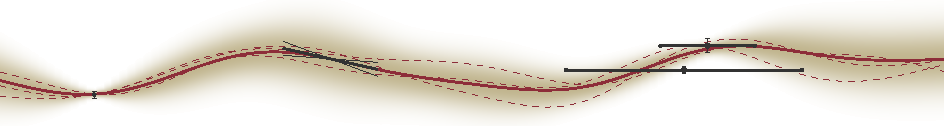
\includegraphics[width=0.9995\paperwidth]{assets/logo_TU_169_0.pdf}
  \end{columns}
  %%%%%%%%%%%%%% END OF ANIMATED LOGO %%%%%%%%%%%

\end{frame}
\tikzexternalenable

\setlength{\figwidth}{.9\textwidth}
\setlength{\figheight}{.6\textheight}


%%%%%%%%%%%%%%%% Intro  %%%%%%%%%%%%%%%%

\begin{frame}\frametitle{Introduction}
    \framesubtitle{Why Classification of Emotions?}
    
\begin{columns}
	
	\column{.6\textwidth}
    
\emph{Emotions:}
\begin{figure}
	\includegraphics[width=.7\textwidth]{figures/2DemotionMapping.pdf}	
	\caption{A two-dimensional emotion space with an Arousal and a Valence axis. Basic emotions are marked as ellipses within the quadrant. }

\end{figure}
   
	%\includegraphics[scale=0.9]{2DemotionMapping.pdf}
\vspace{2em}
\column{.5\textwidth}
\vspace{1em}
	\emph{Different Databases to classify emotions on:}
	\vspace{1em}
	\begin{figure}
		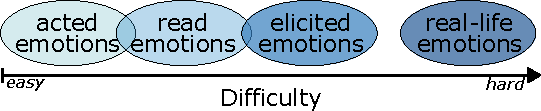
\includegraphics[width=1.0\textwidth]{figures/differentDatabases.pdf}	
		\caption{Types of databases used for emotion recognition and their difficulty.}
	\end{figure}


	
	\end{columns}
\end{frame}

%%%%%%%%%%%%%%%% Intro  %%%%%%%%%%%%%%%%



%%%%%%%%%%%%%%%% Intro  %%%%%%%%%%%%%%%%

\begin{frame}\frametitle{Introduction}
    \framesubtitle{How to Process Emotions?}
    


\vspace{2em}

\vspace{1em}
	\emph{Automatic Speech Emotion Recognition System:}
	\begin{figure}
	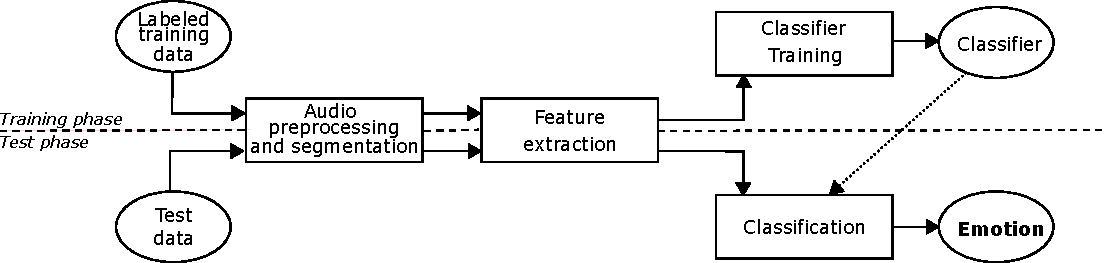
\includegraphics[width=\textwidth]{figures/EmotionRecognitionSystem.pdf}
	\caption{Overview of speech emotion recognition system.}
\end{figure}


	

\end{frame}


%%%%%%%%%%%%%%%% Speech basics  %%%%%%%%%%%%%%%%

\begin{frame}\frametitle{Emotions}
    \framesubtitle{How are you feeling?}
    


\vspace{2em}

\vspace{1em}
	\emph{Acoustic Properties in Speech:}

	\small
	\begin{table}
		%\tablepreamble
		\newcolumntype{Y}{>{\centering\arraybackslash}X}
		\renewcommand{\arraystretch}{1.1}
		\centering
		\caption[]{Some variations of acoustic variables observed in relation to emotions, from \cite{vogt2008automatic}.}
		
		\begin{tabularx}{\textwidth}{YYYYY}
			\toprule
			\textbf{Emotion}&  \textbf{Pitch} &  \textbf{Intensity} &  \textbf{Speaking Rate}&\textbf{Voice Qualtiy}  \\
			\midrule
			\rowcolor{tblhead}
			Anger & high mean, wide range& increased& increased &breathy; blaring timbre \\
			Joy & increased mean and range & increased &increased &sometimes breathy; moderately blaring timbre\\
			\rowcolor{tblhead}
			Sadness & normal or lower than normal mean, narrow range & decreased & slow& resonant timbre  \\
			\bottomrule
		\end{tabularx}
	\end{table}
	
	

\end{frame}





%%%%%%%%%%%%%%%% Dataset  %%%%%%%%%%%%%%%%


\begin{frame}\frametitle{Data Processing}
    \framesubtitle{How did you feel?  \hspace*{30em} \href{https://zenodo.org/record/1188976}{Dataset: https://zenodo.org/record/1188976}}
    
    \vspace{1.5em}


  
	\begin{columns}
		\column{.6\textwidth}
		\begin{figure}
			\centering
			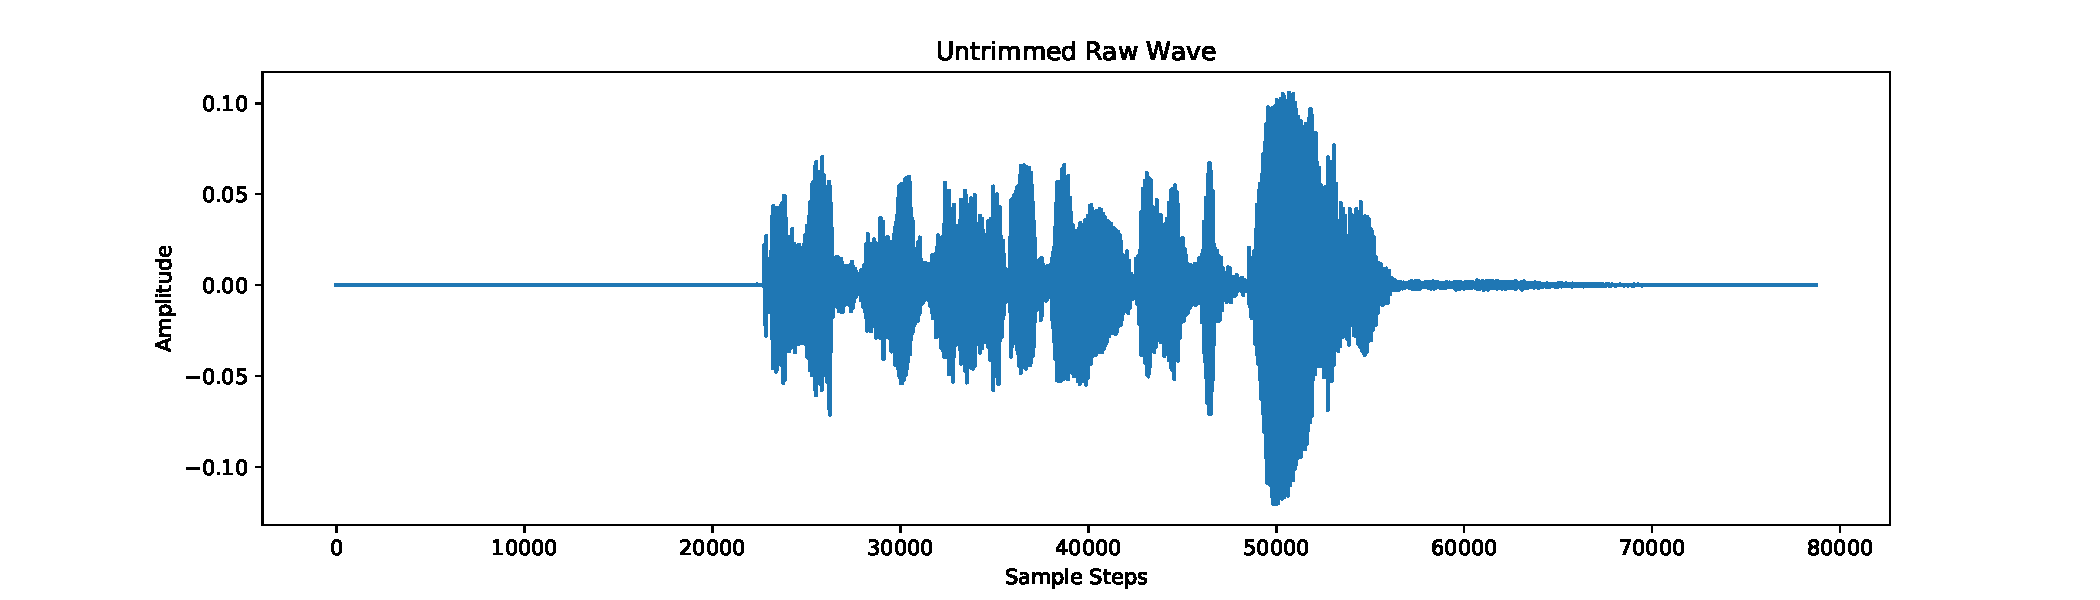
\includegraphics[width=.8\textwidth]{figures/untr_raw_wave.pdf}
			\caption{Un-trimmed sound wave of woman saying 'Dogs are sitting by the door.' in an fearful manner. There is still a lot of meaningless silence before and after the woman speaking. }
			\label{fig:untrimmed sw}
		\end{figure}
		\column{.5\textwidth}
\emph{Dataset}
\begin{itemize}
	\item \textit{Ryerson Audio-Visual Database of Emotional Speech and Song} (RAVDESS)
	\item The RAVDESS database 'is a validated multimodal database of speech and song 
	\item  24 professional actors and actresses, equally balanced in gender, were recorded phrasing main clauses such as  'Dogs are sitting by the door.' 
	\item  North American English 
	\item in one of the following eight emotions: neutral, calm, happy, sad, angry, fearful, disgust, surprised.
	\item  1440 RAVDESS files used  (audio-only) 
	
\end{itemize}
	\end{columns}


\end{frame}



%%%%%%%%%%%%%%%% Software and Applications %%%%%%%%%%%%%%%%
\begin{frame}\frametitle{Data Preprocssing}
    \framesubtitle{Turning speech into numbers ...}
	\begin{columns}
	
		\column{.5\textwidth}
	
	
		\emph{Audio Preprocessing ...}
		
	
		
		
		
		
		%TODO add explanation to equation parts
		
		\column{.5\textwidth}
	
		\emph{Speech Processing:}
		
		
		
	
		\end{columns}
	\end{frame}



% %%%%%%%%%%%%%%%% Evaluation Metrics %%%%%%%%%%%%%%%
%  \begin{frame}\frametitle{Evaluation Metrics}
%     \framesubtitle{How did the Model perform?}

% 	\begin{columns}
	
%  	\column{.5\textwidth}
	
% 	\emph{Confusion Matrix:}\\
% 	{\small The number of correct and incorrect predictions is summarized in a confusion matrix, from which evaluation metrics can be derived.}
%  	\vspace{-.9em}
% 	\begin{figure}
% 		%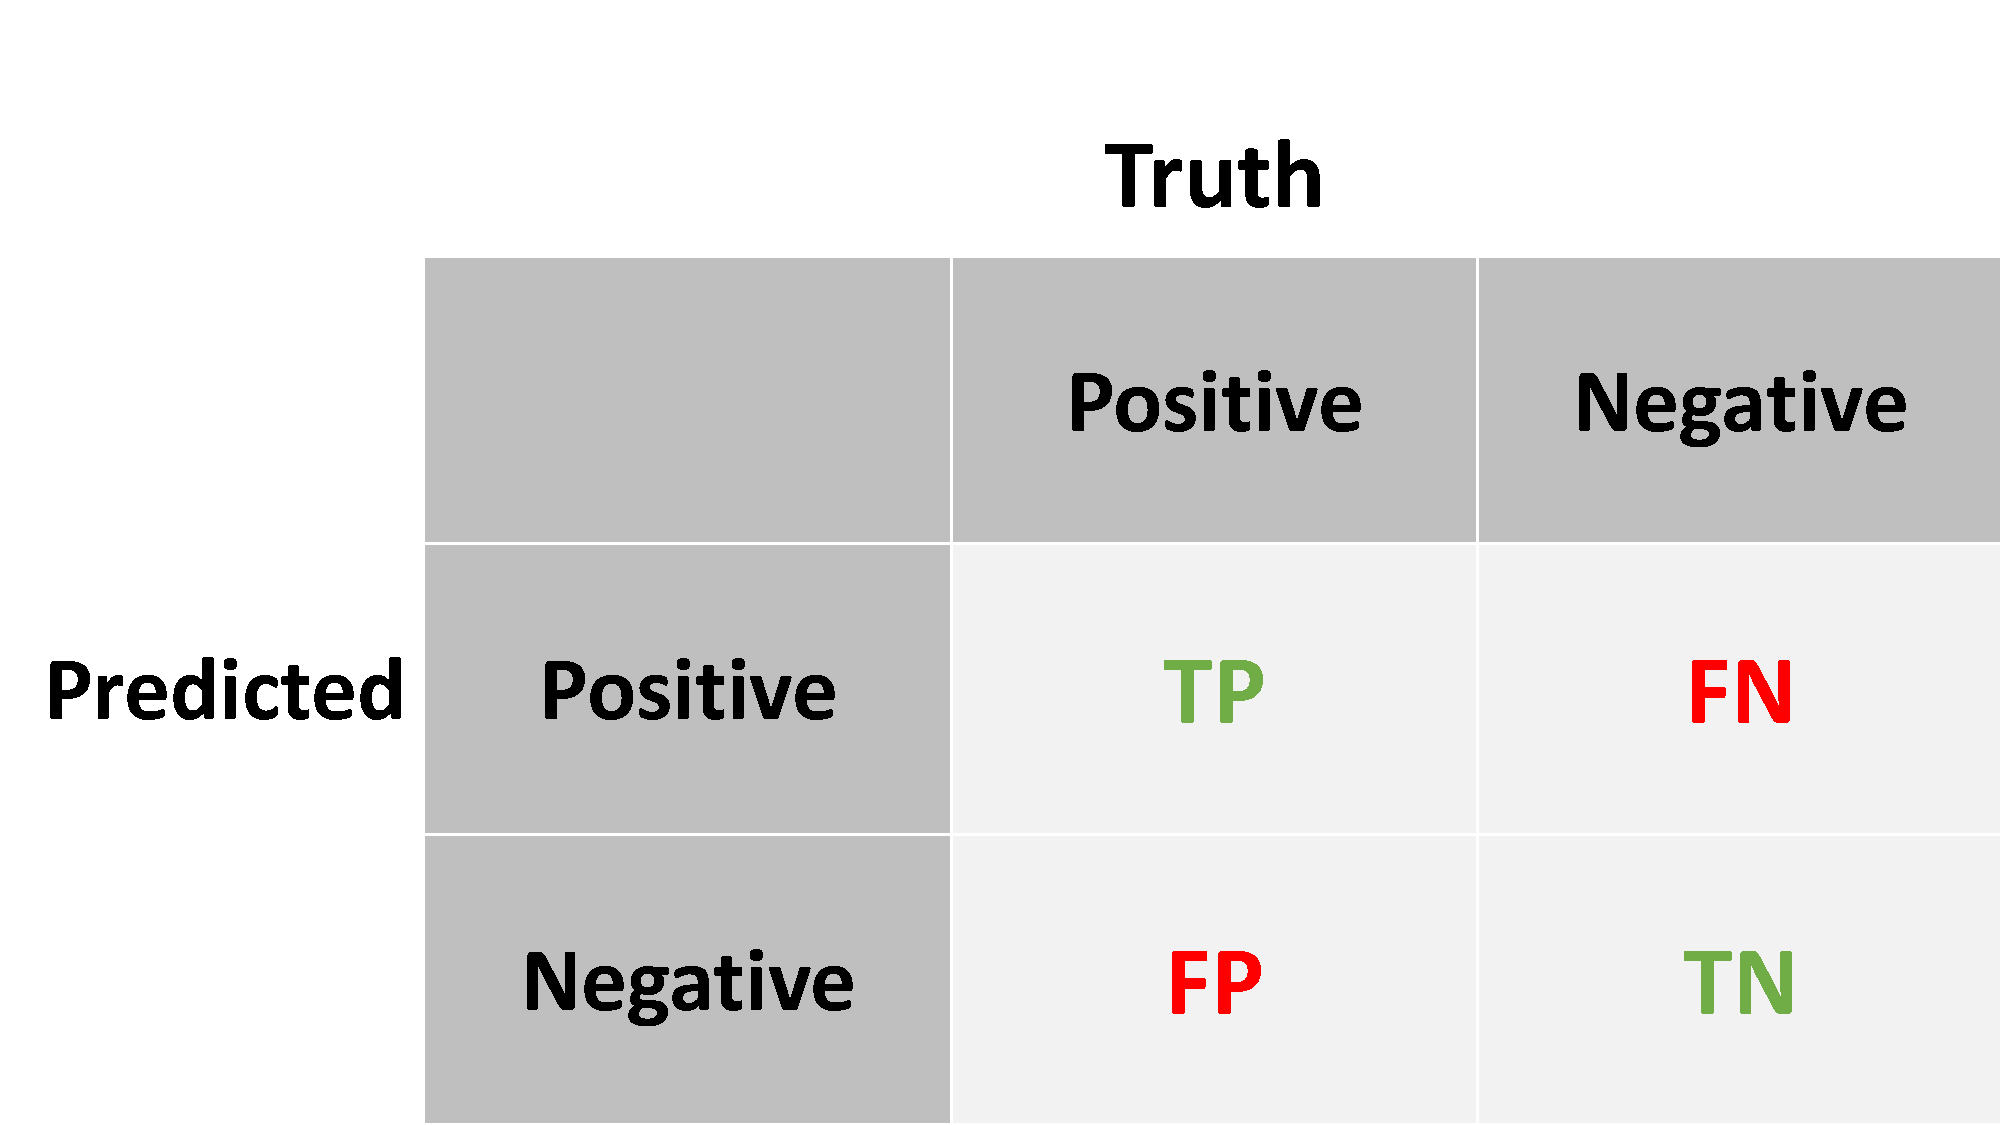
\includegraphics[scale =.1]{figures/confusion-matrix.pdf}
% 		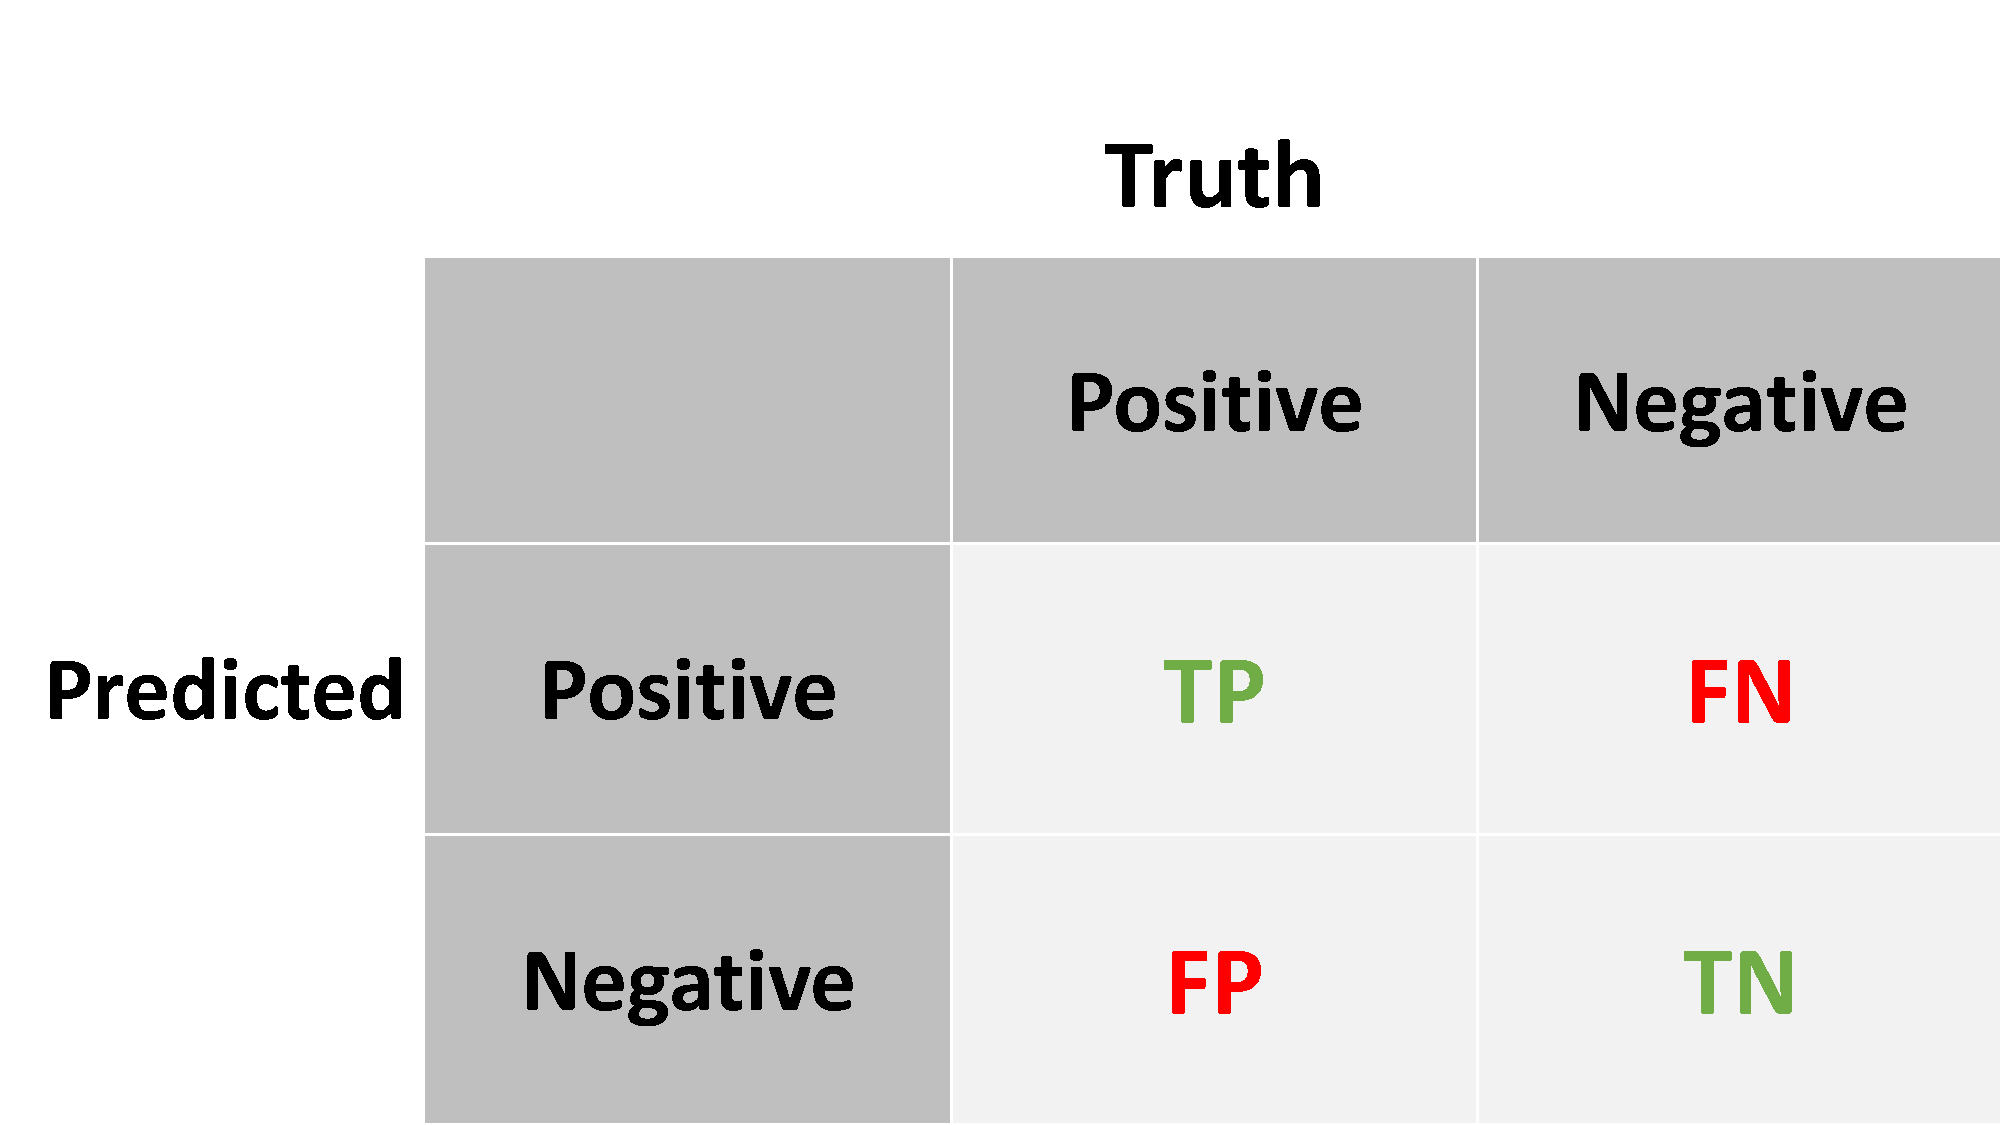
\includegraphics[width=.7\textwidth]{figures/confusion-matrix.pdf}

% 		%\caption{Confusion Matrix.}
% 	\end{figure}
	
% 	\vspace{.5em}
% 	\emph{Evaluation Metrics ...}
% 	{\small
% 	\begin{itemize}
% 		\item accuracy
% 		\item  recall
% 		\item precision
% 		\item F-score.
% 	  \end{itemize}}

%  	\column{.5\textwidth}
% 	 \makebox[\linewidth]{\color{TUgray}{\rule{\textwidth}{2pt}}}
% 	  \small{
%  	 \emph{Accuracy:} Proportion of correct classifications.
% 	 %$ \frac{TP + TN}{TP + TN + FP + FN}$\\
% 	 $ \frac{TP + TN}{\text{Total}}$\\
% 	 ... does not convey a lot of information on the model's performance.
% 	 \makebox[\linewidth]{\color{TUgray}{\rule{\textwidth}{2pt}}}
% 	%\vspace{1em}
	
% 	 \emph{Recall(+)} 
% 	 $ =\frac{TP}{TP + FN}$ \\
% 	 Proportion of \textit{correct positive} classifications from cases that are \textit{actually positive}. \\

% 	 \vspace{1em}	
% 	 \emph{Recall(-)} $ = \frac{TN}{TN + FP}$\\
% 	% Proportion of \textit{correct negative } classifications from cases that are \textit{actually negative}. \\
% 	 \vspace{1em}	
% 	 \emph{Precision(+):} 
% 	 $ \frac{TP}{TP + FP}$ \\
% 	 Proportion of \textit{correct positive} classifications from cases that are \textit{predicted as positive}. \\

% 	\vspace{1em}	
%  		\emph{Precision(-):}
% 	  $  \frac{FN}{FN + TN}$\\
% 	 % \vspace{1em}	

% 	  \makebox[\linewidth]{\color{TUgray}{\rule{\textwidth}{2pt}}}

% 	  \emph{F-Score:}
% 	  $F_{\beta} = \frac{(1- \beta^2) \cdot \text{Precision}  \cdot \text{Recall}}{\beta^2 \cdot \text{Precision}  \cdot \text{Recall}}$
% 	  } \\
% 	  ... a combination of recall and precision.
% 	  \makebox[\linewidth]{\color{TUgray}{\rule{\textwidth}{2pt}}}\\


% 	\end{columns}
%  \end{frame}

%%%%%%%%%%%%%%%%%%%%%%%%%%%%%%%

% \begin{frame}\frametitle{Feature Extraction}
% 	\framesubtitle{ ... }% \hspace*{38em} [2] \href{https://aipoint.tech}{aipoint.tech}}
% %  \framesubtitle{What was the movie like?  \hspace*{33em} \href{https://www.rottentomatoes.com}{www.rottentomatoes.com}}

	
	
	
	
% \end{frame}

%%%%%%%%%%%%%%%%  %%%%%%%%%%%%%%%%
\begin{frame}\frametitle{Classification Algorithms}
    \framesubtitle{(1) Convolutional Neural Network}

	\begin{columns}
	
		\column{.7\textwidth}
		\vspace{2em}
		\begin{itemize}
			\item CNNs are a special kind of neural network
			\item inspired by the concept of the mammalian retina
			\item have proven to perform well on high-dimensional input 
			\item use convolution as a specialized kind of linear operation in place of a general matrix multiplication
			\item Advantageous to CNNs is their high efficiency in terms of  computational complexity while using a sparse set of parameters
			\item The kernels which the CNN learns during training process, are reused over the entire input which markedly exceeds regular feed forward networks in terms of memory and computational efficiency.


		\end{itemize}
		
		
   \column{.3\textwidth}

		\end{columns}
	\end{frame}


%%%%%%%%%%%%%%%%  %%%%%%%%%%%%%%%%
\begin{frame}\frametitle{Classification Algorithms}
    \framesubtitle{(2) Support Vectore Machine}

	\begin{columns}
		\vspace{1em}
		\column{.5\textwidth}
	
		\emph{Support Vector machine:}
		\begin{itemize}
			\item \textbf{Goal:}  find a hyperplane of the form $\mathcal{H} = \left\lbrace x \in \mathbb{R}^d | \left\langle w,x\right\rangle + b =0 \right\rbrace $ such that it separates the data while maximizing the distance between the hyperplane and the closest data point. 
			\item This distance is referred to as the margin. 
			\item By maximizing the margin, the classifier is most robust to noise in new data
		\end{itemize}
		\vspace{1em}

\column{.6\textwidth}


\begin{figure}
	\centering
	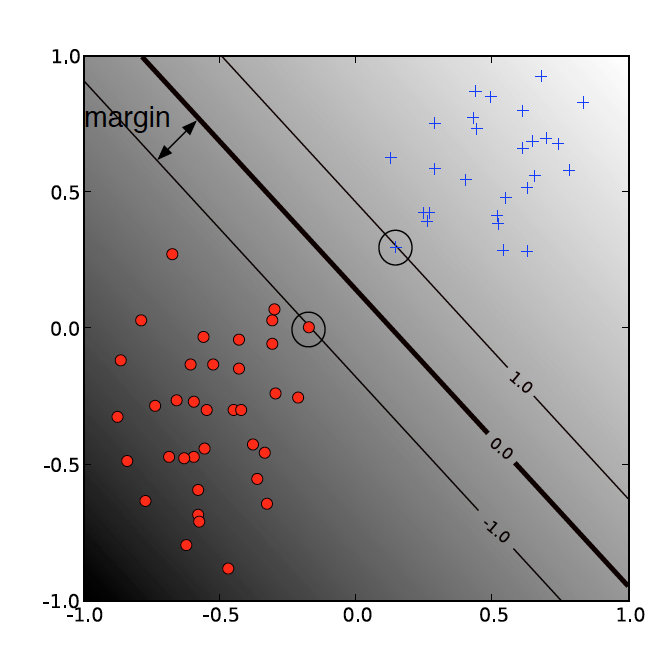
\includegraphics[width=0.6\textwidth]{figures/svm.png}
	\caption{A linear SVM. The circled data points are the \textit{support vectors} -- i.e., the examples that are closest to the decision boundary. The support vectors determine the the margin with which the two classes are separated. In this work, eight classes need to be separated.}

\end{figure}
		
		\end{columns}
	\end{frame}




%%%%%%%%%%%%%%%% Results %%%%%%%%%%%%%%%%
\begin{frame}\frametitle{Results}
    \framesubtitle{Who did better?}
	\begin{columns}
	
		\column{.5\textwidth}
	


		
		\vspace{0.5em}
	
\emph{SVM-Model Parameters:}
		\begin{align*}
			l = 745 \qquad &\text{(number of principal components of PCA)}\\
			\gamma_{\text{\tiny PCA}} =  1 \qquad &\text{(inversed kernel width of PCA)}\\
			C = 10 \qquad &\text{(soft-margin constant of SVM)}\\
			\gamma_{\text{\tiny SVM}} = 10 \qquad &\text{(inversed kernel width of SVM)}
			\end{align*}

\vspace{1em}
		\vspace{.1em}
		\column{.5\textwidth}
	
		\emph{Comparison }
		%{\small
		\begin{table}[htbp]
		  \centering
		  \label{tbl:timeline}
		  \begin{tabular}{l c c}
			\toprule
			SVM&  Training& Test\\
			\midrule
			Accuracy & $ 97.05\%$ & $63.39\%$\\
			
		  
			\bottomrule
		  \end{tabular}
		  \caption{Results of evaluating the SVM-model on the training and  test data.}
		  \end{table}%}

		  $\rightarrow$ %\textbf{LR} ( $F=86.8\%$) outperforms \textbf{NB} ( $F =45.3\%$) 
		\end{columns}

	
		
	\end{frame}


	%%%%%%%%%%%%%%%% Bigger picture  %%%%%%%%%%%%%%%%

% \begin{frame}\frametitle{Let's Zoom out ...}
%     \framesubtitle{Recommender Systems}
    
%     \vspace{1.5em}
    
%     	\begin{center}
%     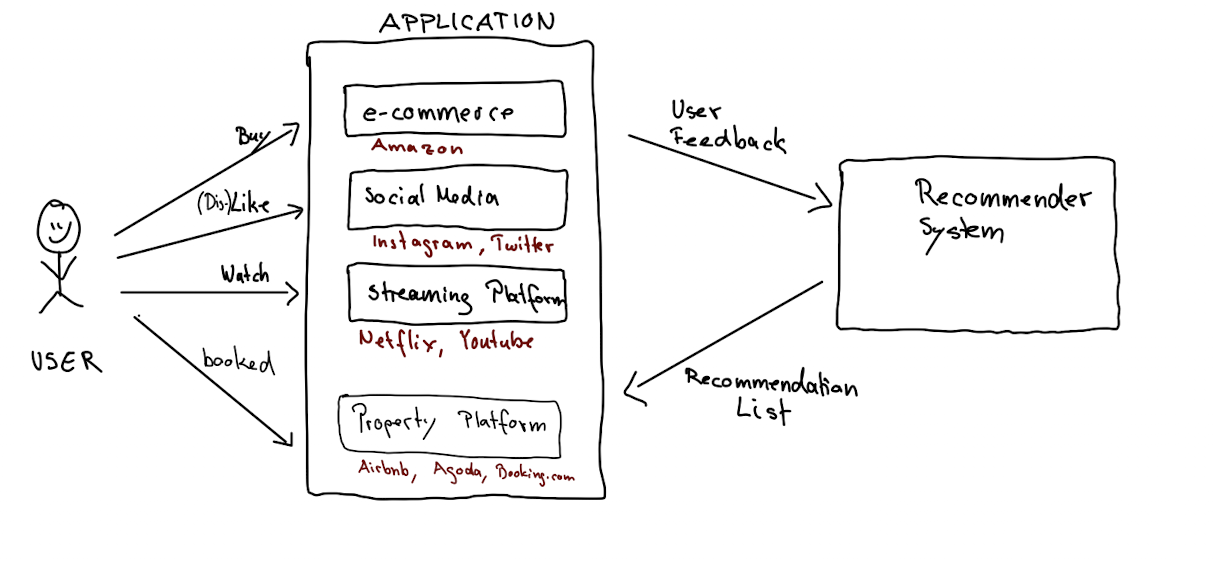
\includegraphics[width=.8\textwidth]{figures/recommender-system.png}	
% 		\end{center}

% 		\vspace{.5em}
    
% 		\begin{center}
% 			\emph{Objectives from Application's point of view:} \\
% 			\textbullet	\, maximize revenue \quad \textbullet	\,maximize user's time spent on platform  
% 		\end{center}

% \end{frame}

% %%%%%%%%%%%%%%%% bigger picture  %%%%%%%%%%%%%%%%


% \begin{frame}\frametitle{Bigger Picture }
%     \framesubtitle{What was your experience like?}
    
%     \vspace{1.5em}
% \begin{columns}
% 	\column{.8\textwidth}
    
%     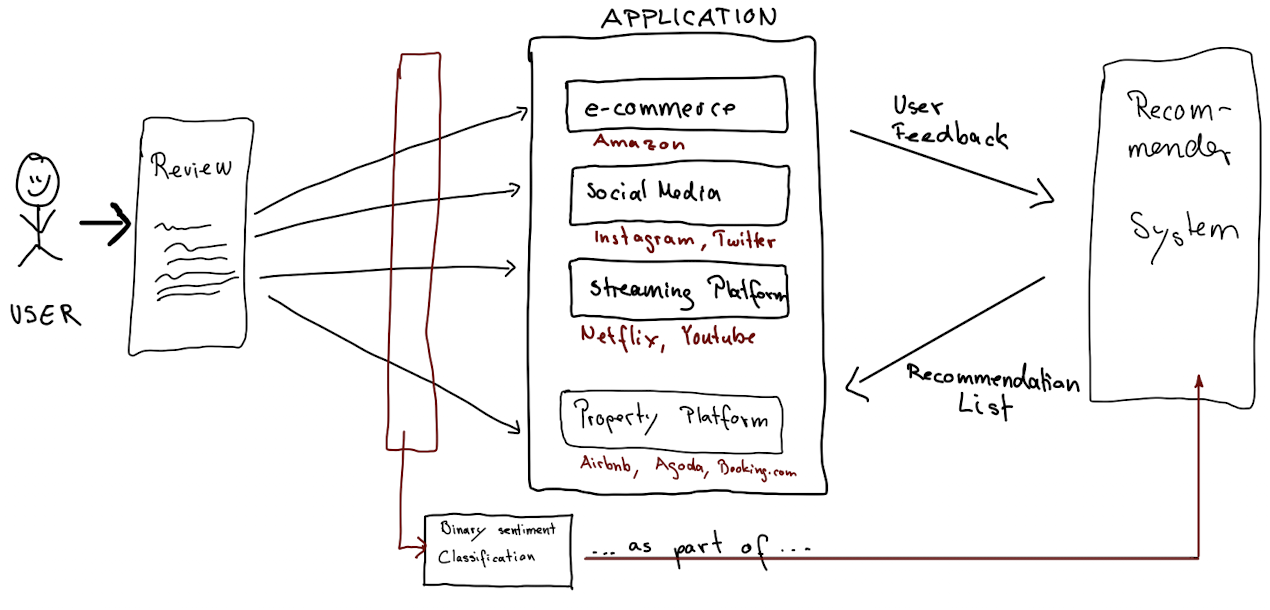
\includegraphics[width=.95\textwidth]{figures/recommender-system-sentiment-classification.png}	
	

% 		\vspace{.5em}

% 		\column{.3\textwidth}
%     	\emph{Sentiment Classification as part of a Recommender System: } \\
% 		\begin{itemize}
% 			\item here: based on movie reviews
% 			\item binary classification
% 		\end{itemize}


% 	\end{columns}
% \end{frame}





%%%%%%%%%%%%%%%%%%%% SUMMARY

\blackslidetext{
	\frametitle{\emph{Summary}}
	
	\begin{columns}
		
	\column{.5\textwidth}
\textbf{SVM:}
\vspace{-.6em}
	{\small
	\begin{table}[htbp]
		\centering
		\label{tbl:timeline}
		\begin{tabular}{l c c}
		  \toprule
		  SVM&  Training& Test\\
		  \midrule
		  Accuracy & $ 97.05\%$ & $63.39\%$\\
		  
		
		  \bottomrule
		\end{tabular}
		%\caption{Results of evaluating the SVM-model on the training and  test data.}
		\end{table}}
		  \vspace{.6em}

	\textbf{CNN:}\\

	{\small
	\begin{itemize}
		\item did not learn the problem at all
		\item probably training data too small
		\item $\rightarrow$ was not further pursued
	\end{itemize}}


	
	\column{.5\textwidth}
	\vspace{3em}
	\textbf{Improvements:}
	\vspace{-3em}
	{\small
	\begin{itemize}
		\item incorporate transcribed text data
		\item include videos to have facial expressions as additional feature
		\item using the validation set to find better hyperparameters
		\item $\rightarrow$ would make a plethora of established  methods used in text processing available.
\begin{itemize}
	\item feature extracting with BoW- or tf-idf method
	\item n-grams to capture context of a word
\end{itemize}
	\end{itemize}}
	\end{columns}
	\vspace{.5em}
	\begin{center}
		\makebox[\linewidth]{\color{TUgray}{\rule{\textwidth}{2pt}}}
		\LARGE \emph{Thank You!}
		\makebox[\linewidth]{\color{TUgray}{\rule{\textwidth}{2pt}}}
	\end{center}
	

}
  


%%%%%%%%%%%%%%%% HOW TO .... %%%%%%%%%%%%%%%%
% \begin{frame}\frametitle{How to ...}
%     \framesubtitle{?}

% 	\makebox[\linewidth]{\color{TUgray}{\rule{\textwidth}{2pt}}}
	
% 	\begin{columns}
	
% 	\column{.2\textwidth}
% 	\centering
% 	\includegraphics[width=0.8\textwidth]{figures/pn_logo.png}
		
% 	\column{.75\textwidth}
% 	\vspace{0.25em}
	
% 	{\small \textbf{ProbNum} implements probabilistic numerical methods in Python.
% 	\begin{center}
% 	\url{https://github.com/probabilistic-numerics/probnum}
% 	\end{center}
% 	or alternatively \colorbox{lgra}{\texttt{pip install probnum}}.
% 	}
% 	\vspace{0.25em}
% 	\end{columns}
	
% 	\makebox[\linewidth]{\color{TUgray}{\rule{\textwidth}{2pt}}}

% 	\vspace{1em}

% 	\emph{Future Applications}
% 	\begin{center}
%     \begin{tabular}{cc}
% 	\includegraphics[width=.23\textwidth]{figures/PDE_solution_samples.pdf}
% 	\includegraphics[width=.15\textwidth]{figures/PDE_fine_solution.pdf} &
% 	\includegraphics[width=.275\textwidth]{figures/nonconvex_surface.png}\\
%     Galerkin Methods \(\mA \vu = \vf\)&
%     Empirical Risk Minimization \(\rmH \vd = \rvg\)
%     \end{tabular}
%     \end{center}

% \end{frame}   

%% References
%\newcounter{references}
%\setcounter{references}{\value{framenumber}} % Adjust frame counter to not include references
%
%\begin{frame}[allowframebreaks]{References}
%\bibliographystyle{plainnat}
%\bibliography{references}
%\end{frame}
%
%\setcounter{framenumber}{\value{references}}


\end{document}